\documentclass[10pt]{article}
\usepackage[margin=0.65in]{geometry}\usepackage{amsmath,amssymb,tikz,hyperref}\setlength{\parindent}{0pt}\setlength{\parskip}{5pt}
\begin{document}
\textbf{Frozen scalar-projection input audit}\hfill 2026-10-31\\T-1125. Producer metadata audit; independent review pending.
\section*{Recorded results}
Nine frozen plan hashes match the reconciliation index. The eight enrollment plans contain \textbf{1,260 distinct workload IDs}, grouped into 21 curve metadata identities (60 targets each). A separate one-target gate stays outside these totals. All 1,261 metadata records pass: order divisibility by $r$, cofactor agreement, duplicate order/$r$ field agreement, Hasse interval containment, and $r>4p$. Every supplied cofactor is coprime to $r$.
\begin{center}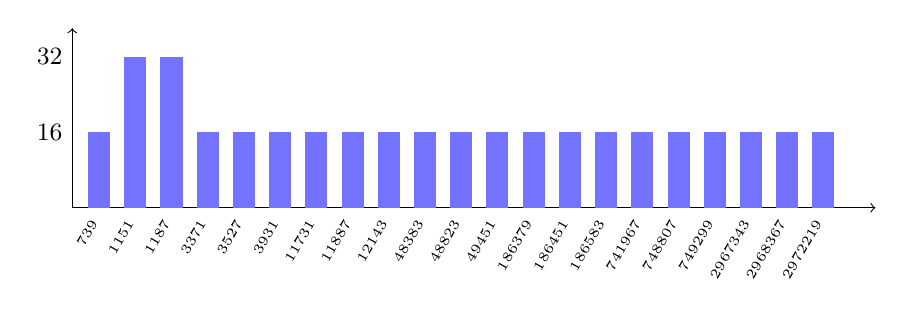
\begin{tikzpicture}[x=1cm,y=0.6cm]
\draw[->] (-.2,0)--(10,0);\draw[->] (-.2,0)--(-.2,3.8);
\node[anchor=east,font=\small] at (-.2,1.6) {16};\node[anchor=east,font=\small] at (-.2,3.2) {32};
\fill[blue!55] (0.0,0) rectangle (0.28,1.6);\node[font=\tiny,rotate=60,anchor=east] at (0.14,-0.1) {739};
\fill[blue!55] (0.46,0) rectangle (0.74,3.2);\node[font=\tiny,rotate=60,anchor=east] at (0.6000000000000001,-0.1) {1151};
\fill[blue!55] (0.92,0) rectangle (1.2000000000000002,3.2);\node[font=\tiny,rotate=60,anchor=east] at (1.06,-0.1) {1187};
\fill[blue!55] (1.3800000000000001,0) rectangle (1.6600000000000001,1.6);\node[font=\tiny,rotate=60,anchor=east] at (1.52,-0.1) {3371};
\fill[blue!55] (1.84,0) rectangle (2.12,1.6);\node[font=\tiny,rotate=60,anchor=east] at (1.98,-0.1) {3527};
\fill[blue!55] (2.3000000000000003,0) rectangle (2.58,1.6);\node[font=\tiny,rotate=60,anchor=east] at (2.4400000000000004,-0.1) {3931};
\fill[blue!55] (2.7600000000000002,0) rectangle (3.04,1.6);\node[font=\tiny,rotate=60,anchor=east] at (2.9000000000000004,-0.1) {11731};
\fill[blue!55] (3.22,0) rectangle (3.5,1.6);\node[font=\tiny,rotate=60,anchor=east] at (3.3600000000000003,-0.1) {11887};
\fill[blue!55] (3.68,0) rectangle (3.96,1.6);\node[font=\tiny,rotate=60,anchor=east] at (3.8200000000000003,-0.1) {12143};
\fill[blue!55] (4.140000000000001,0) rectangle (4.420000000000001,1.6);\node[font=\tiny,rotate=60,anchor=east] at (4.28,-0.1) {48383};
\fill[blue!55] (4.6000000000000005,0) rectangle (4.880000000000001,1.6);\node[font=\tiny,rotate=60,anchor=east] at (4.74,-0.1) {48823};
\fill[blue!55] (5.0600000000000005,0) rectangle (5.340000000000001,1.6);\node[font=\tiny,rotate=60,anchor=east] at (5.2,-0.1) {49451};
\fill[blue!55] (5.5200000000000005,0) rectangle (5.800000000000001,1.6);\node[font=\tiny,rotate=60,anchor=east] at (5.66,-0.1) {186379};
\fill[blue!55] (5.98,0) rectangle (6.260000000000001,1.6);\node[font=\tiny,rotate=60,anchor=east] at (6.12,-0.1) {186451};
\fill[blue!55] (6.44,0) rectangle (6.720000000000001,1.6);\node[font=\tiny,rotate=60,anchor=east] at (6.58,-0.1) {186583};
\fill[blue!55] (6.9,0) rectangle (7.180000000000001,1.6);\node[font=\tiny,rotate=60,anchor=east] at (7.04,-0.1) {741967};
\fill[blue!55] (7.36,0) rectangle (7.640000000000001,1.6);\node[font=\tiny,rotate=60,anchor=east] at (7.5,-0.1) {748807};
\fill[blue!55] (7.82,0) rectangle (8.1,1.6);\node[font=\tiny,rotate=60,anchor=east] at (7.96,-0.1) {749299};
\fill[blue!55] (8.280000000000001,0) rectangle (8.56,1.6);\node[font=\tiny,rotate=60,anchor=east] at (8.420000000000002,-0.1) {2967343};
\fill[blue!55] (8.74,0) rectangle (9.02,1.6);\node[font=\tiny,rotate=60,anchor=east] at (8.88,-0.1) {2968367};
\fill[blue!55] (9.200000000000001,0) rectangle (9.48,1.6);\node[font=\tiny,rotate=60,anchor=east] at (9.340000000000002,-0.1) {2972219};
\end{tikzpicture}\end{center}
\small Chart: supplied cofactor (dimensionless) against field parameter $p$, from \texttt{curves.json}. Nineteen curve identities have cofactor 16; two have 32. Metadata only, no sampling uncertainty.\normalsize
\section*{Upstream guard located}
The ecbench workload builder constructs \texttt{StudyInstance} then calls its validator (\texttt{workload.rs:268--305}). In the engine (\texttt{three\_leads.rs}, lines 1308--1370), the validator checks prime $r$, $rh=\mathrm{order}$, $r\nmid h$, valid nonzero generator and $[r]P=0$. Thus the broader construction path includes the coprimality guard absent from the earlier local solver excerpt. Direct solver callers still need their own input contract.

Given a nonzero point of prime order $r$, the true elliptic order is divisible by $r$. Its Hasse interval over $\mathbf F_{p^2}$ has width $4p$; if $r>4p$, it contains at most one multiple of $r$. The source uses this strategy. This audit checks supplied interval arithmetic, not the point or primality witness. Identifying that order with the destination Jacobian still needs the bound isogeny argument.
\section*{Transfer evidence and next binding}
The existing test \texttt{quadratic\_fields\_and\_transfer} checks $\operatorname{norm}(\tau(P))=[2]P$ for all enumerated points in eight small fields, plus 100 sampled additivity pairs per field. This describes test source, not a fresh execution or the 21 cohort fields. A universal norm--tau identity would establish nonzero transfer for a nonzero point of odd prime order. Bind that identity and the destination cardinality to the actual implementation next.
\section*{Custody and scope}
\texttt{PLAN.md} precedes the audit; \texttt{audit.py} hashes inputs before parsing. \texttt{rows.jsonl} preserves 1,261 metadata rows, excluding planted scalars and target coordinates. Source and input hashes are retained. No prime check, point count, transfer replay, target generation, timing or scientific workload was run. Cost ratio is null; expired campaign limits are unchanged.

Source reading: the bound repository files and previous scalar-coordinate derivation. Primary reference: \href{https://doc.sagemath.org/html/en/reference/arithmetic_curves/sage/schemes/elliptic_curves/ell_finite_field.html}{Sage finite-field elliptic curve documentation}, \texttt{has\_order}/\texttt{set\_order}, distinguishes sanity checks from stronger order evidence. Sage was not run; ecdb tool unavailable.
\end{document}
